\documentclass[border=5pt]{standalone}
\usepackage{tikz}
\usetikzlibrary{arrows.meta}

\tikzset{
  >={Latex[width=1mm,length=2mm]},
  % Specifications for style of nodes:
            base/.style = {rectangle, rounded corners, draw=black,
                           minimum width=4cm, minimum height=1cm,
                           text centered, font=\sffamily},
  activityStarts/.style = {base, fill=blue!30},
       startstop/.style = {base, fill=red!30},
    activityRuns/.style = {base, fill=green!30},
         process/.style = {base, minimum width=2.5cm, fill=orange!15,
                           font=\ttfamily},
}
\begin{document}    
% Drawing part, node distance is 1.5 cm and every node
% is prefilled with white background
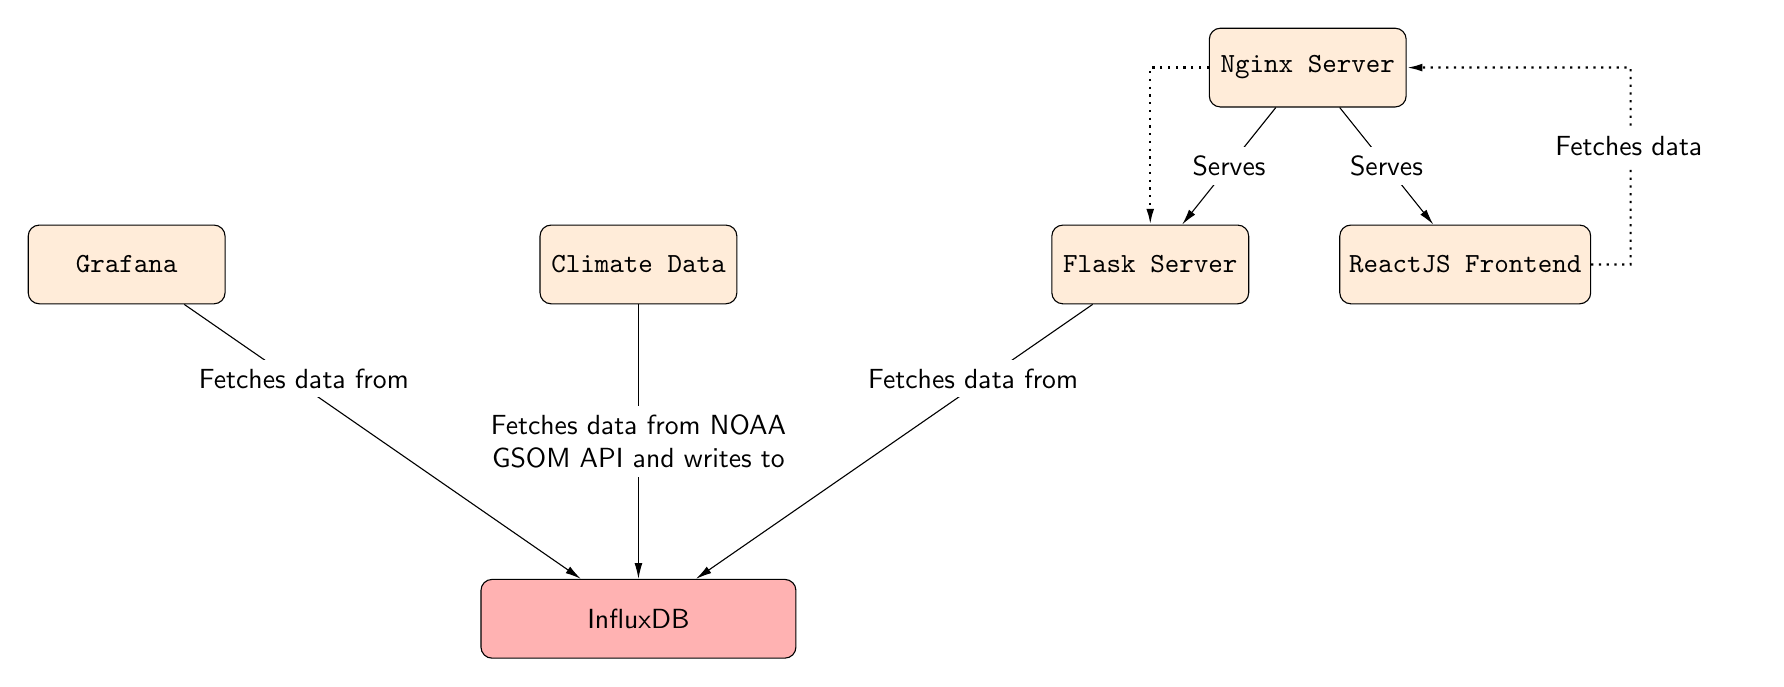
\begin{tikzpicture}[node distance=2.5cm,
      every node/.style={fill=white, font=\sffamily}, align=center]
    % Specification of nodes (position, etc.)
    \node (nginxServer)       [process]                     {Nginx Server};
    \node (react)             [process, below of=nginxServer, xshift=2cm]
                                                        {ReactJS Frontend};
    \node (flask)             [process, below of=nginxServer, xshift=-2cm]
                                                            {Flask Server};
    \node (climateData)       [process, left of=flask, xshift=-4cm]
                                                            {Climate Data};
    \node (grafana)           [process, left of=climateData, xshift=-4cm]
                                                                 {Grafana};
    \node (influx)            [startstop, below of=climateData, yshift=-2cm]
                                                                {InfluxDB};
    
    
    % Specification of lines between nodes specified above
    % with aditional nodes for description 
    \draw[->]                       (nginxServer) -- node[text width=2cm]
                                                        {Serves} (flask);
    \draw[->]                       (nginxServer) -- node[text width=2cm]
                                                        {Serves} (react);
    \draw[->, dotted, thick]        (react.east)  -- ++(0.5, 0) -- ++(0, 2.5) -- 
                                     node[yshift=-1cm, xshift=1.4cm, text width=3cm]
                                                       {Fetches data} (nginxServer);
    \draw[->, dotted, thick]        (nginxServer) -| (flask);
    \draw[->]                       (flask) -- node[xshift=1cm, yshift=.8cm, text width=4cm]
                                                              {Fetches data from} (influx);
    \draw[->]                       (grafana) -- node[xshift=-1cm, yshift=.8cm, text width=4cm]
                                                                    {Fetches data from} (influx);
    \draw[->]                      (climateData) -- node[text width=4cm]
                                   {Fetches data from NOAA GSOM API and writes to} (influx);


  \end{tikzpicture}
\end{document}